% ----------------------------------------------------
\begin{frame}
  \titlepage
\end{frame}
% ----------------------------------------------------
\note{Introducción a la sesión. Conectar con la sesión anterior sobre comercio. Hoy pasamos del flujo de bienes al flujo de dinero y capital: la otra cara de la economía política internacional. Las finanzas internacionales son quizás la dimensión más técnica de la política mundial, pero también una de las más políticamente explosivas. Las crisis financieras han derrocado gobiernos, impuesto austeridad sobre millones de personas, y reconfigurado la política doméstica de países enteros. Cuatro grandes bloques: inversión internacional, deuda soberana, tipos de cambio, y crisis monetarias.}

% ----------------------------------------------------
\begin{frame}
\frametitle{Hoy}
\centering
\vspace{1.5em}
\begin{itemize}
  \setlength{\itemsep}{10pt}
  \item El rompecabezas: ¿por qué es tan política la financiación internacional?
  \item Inversión internacional: tipos, lógica y multinacionales
  \item Prestamistas y deudores: ganancias, conflictos y el FMI
  \item Tipos de cambio: sistemas y ganadores
  \item Crisis monetarias: Argentina, el euro y el contagio
\end{itemize}
\end{frame}
% ----------------------------------------------------
\note{}

% ====================================================
\section{El rompecabezas}
% ====================================================

% ----------------------------------------------------
\begin{transitionframe}
El rompecabezas de las finanzas internacionales
\end{transitionframe}
% ----------------------------------------------------
\note{}

% ----------------------------------------------------
\begin{frame}[plain]
  \begin{tikzpicture}[remember picture, overlay]
    \node[at = (current page.center), yshift = 0cm] (cover) {%
      \includegraphics[keepaspectratio, height=\paperheight]{../img/trading_floor.jpg}};
  \end{tikzpicture}
\end{frame}
% ----------------------------------------------------
% IMAGE NEEDED: trading_floor.jpg -- fotografía de un parqué bursátil o sala de operaciones de un banco de inversión, preferiblemente con pantallas mostrando gráficos financieros y operadores trabajando; transmite la escala y la velocidad de los mercados financieros globales
\note{Imagen de apertura. Los mercados financieros mueven billones de dólares cada día. Más de 5 billones de dólares se invierten en el extranjero cada año. Esto no es solo un fenómeno económico: detrás de cada flujo de capital hay decisiones políticas, relaciones de poder, y conflictos distributivos. La pregunta central de hoy: si el capital fluye libremente, ¿quién gana, quién pierde, y quién decide las reglas del juego?}

% ----------------------------------------------------
\begin{frame}
\frametitle{El rompecabezas}
\centering

\begin{itemize}
  \item Cada año se invierten \textbf{$\sim$5 billones de dólares} en el exterior
  \vspace{8pt}
  \item<2-> La teoría dice que el capital fluye hacia donde genera \textbf{mayores rendimientos}
  \begin{itemize}
    \item Países pobres: escasez de capital $\rightarrow$ rendimientos altos
    \item Países ricos: abundancia de capital $\rightarrow$ rendimientos bajos
  \end{itemize}
  \vspace{8pt}
  \item<3-> Pero las finanzas internacionales son \alert{políticamente controvertidas}:
  \begin{itemize}
    \item Deuda soberana y austeridad
    \item Crisis cambiarias y colapsos económicos
    \item Multinacionales: ¿quién controla los recursos?
  \end{itemize}
  \item<4-> \textbf{Pregunta central:} ¿quién gana y quién pierde con la integración financiera?
\end{itemize}

\end{frame}
% ----------------------------------------------------
\note{El punto de partida es la escala: 5 billones de dólares de inversión exterior anual es un número que supera el PIB de la mayoría de los países del mundo. La economía predice un flujo de capitales de ricos a pobres (donde escasean y rinden más), pero la realidad es más complicada. Las finanzas internacionales generan conflictos políticos intensos porque los flujos de capital no son neutrales: determinan quién puede crecer, quién tiene que pagar la deuda, qué tipo de cambio favorece a los exportadores o a los importadores, y qué países pueden hacer política económica autónoma. Este es el hilo conductor de la sesión.}

% ====================================================
\section{Inversión internacional}
% ====================================================

% ----------------------------------------------------
\begin{transitionframe}
Inversión internacional
\end{transitionframe}
% ----------------------------------------------------
\note{}

% ----------------------------------------------------
\begin{frame}
\frametitle{Dos tipos de inversión internacional}
\centering
\vspace{0.5em}

{\footnotesize
\begin{adjustbox}{width=\textwidth}
\begin{tabular}{>{\bfseries}p{2.8cm} p{3.5cm} p{3cm}}
 & \textbf{\textcolor{accent}{Inversión en cartera}} & \textbf{\textcolor{accent2}{Inversión extranjera directa}} \\[6pt]
\hline
Qué incluye & Préstamos, bonos, acciones & Fábricas, activos reales \\[5pt]
Control & \textbf{No} --- solo rendimiento & \textbf{Sí} --- control de gestión \\[5pt]
Movilidad & Alta --- puede salir rápido & Baja --- activos físicos \\[5pt]
Quién la hace & Bancos, fondos & Multinacionales \\[5pt]
Riesgo político & Impago, control de capitales & Expropiación, regulación \\[5pt]
\end{tabular}
\end{adjustbox}
}

\vspace{8pt}
\onslide<2->{\small La distinción clave: \alert{control de gestión} vs.\ solo rendimiento financiero}

\end{frame}
% ----------------------------------------------------
\note{La distinción entre inversión en cartera e IED es fundamental para entender los debates políticos sobre la inversión extranjera. La inversión en cartera (bonos soberanos, préstamos bancarios, acciones en bolsa) no da al inversor control sobre las decisiones de la empresa o el gobierno. La IED sí: cuando Toyota construye una fábrica en España, toma decisiones sobre qué producir, cuántos trabajar, si cerrar o ampliar. Por eso la IED es políticamente más sensible: genera debates sobre soberanía económica, empleos, y quién controla los sectores estratégicos. La movilidad también es clave: la inversión en cartera puede salir de un país en minutos (``dinero caliente''), generando crisis de balance de pagos. La IED, al ser activos físicos, no puede moverse con tanta rapidez, lo que da cierta estabilidad.}

% ----------------------------------------------------
\begin{frame}
\frametitle{¿Por qué invertir en el extranjero?}
\centering

\begin{itemize}
  \item \textbf{Lógica Heckscher-Ohlin:} el capital fluye donde es escaso
  \begin{itemize}
    \item Países ricos: capital abundante $\rightarrow$ rendimientos bajos (2--3\%)
    \item Países pobres: capital escaso $\rightarrow$ rendimientos altos (10\%+)
  \end{itemize}
  \vspace{8pt}
  \item<2-> El capital debería fluir masivamente de países ricos a países pobres
  \vspace{8pt}
  \item<3-> \textbf{Pero la realidad es distinta:}
  \begin{itemize}
    \item La mayor parte de la IED va de países ricos a países ricos
    \item EE.UU. $\leftrightarrow$ Europa $\leftrightarrow$ Japón
  \end{itemize}
  \item<3-> \textbf{¿Por qué no fluye más capital a los países pobres?}
  \item<4-> $\rightarrow$ \alert{riesgo político}: expropiación, impago, inestabilidad
\end{itemize}

\end{frame}
% ----------------------------------------------------
\note{La paradoja de Lucas (1990): el economista Robert Lucas señaló que el capital no fluye de países ricos a países pobres en la cantidad que la teoría predice. Si el capital rinde más en India o Nigeria que en EE.UU., ¿por qué no hay un torrente de inversión hacia esos países? La respuesta principal: el riesgo político. Invertir en un país en desarrollo conlleva riesgos que no existen en países ricos: expropiación (el gobierno puede nacionalizar la empresa o el activo), incumplimiento de contratos, corrupción, inestabilidad política, controles de capitales que impiden repatriar beneficios. Para compensar ese riesgo, los inversores exigen rendimientos mucho más altos. El resultado: solo los proyectos con rendimientos extraordinariamente altos atraen capital extranjero a los países más pobres, mientras que la mayoría del capital circula entre países ricos donde el riesgo es bajo.}

% ----------------------------------------------------
\begin{frame}
\frametitle{La IED y las multinacionales}
\centering

\begin{itemize}
  \item La IED la realizan principalmente \textbf{empresas multinacionales} (EMN)
  \vspace{8pt}
  \item Motivaciones de las EMN:
  \begin{itemize}
    \item Acceso a \textbf{mercados}: producir donde se vende (Toyota en EE.UU.)
    \item Acceso a \textbf{recursos}: petróleo, minerales, mano de obra barata
    \item \textbf{Eficiencia}: fragmentar la cadena de producción globalmente
  \end{itemize}
  \vspace{8pt}
  \item<2-> Tendencia reciente: \alert{reshoring} y \alert{friendshoring}
  \begin{itemize}
    \item \textit{Reshoring:} traer producción de vuelta al país de origen
    \item \textit{Friendshoring:} reubicar en países aliados políticamente
    \item CHIPS Act (EE.UU., 2022): subsidios para semiconductores en EE.UU.
    \item Apple traslada producción de China a India
  \end{itemize}
\end{itemize}

\end{frame}
% ----------------------------------------------------
\note{Las empresas multinacionales (EMN) son los actores principales de la IED. En el siglo XX, la narrativa dominante era que las EMN buscaban mano de obra barata en países en desarrollo. Hoy el patrón es más complejo: (1) Muchas EMN invierten en países ricos para acceder a sus mercados (no pueden exportar todo desde casa). (2) Las cadenas de valor globales han fragmentado la producción: un iPhone se diseña en EE.UU., tiene chips de Taiwan, pantallas de Corea del Sur, y se ensambla en China. (3) La pandemia del COVID-19 y las tensiones geopolíticas con China han desencadenado un debate sobre la vulnerabilidad de estas cadenas. El reshoring y friendshoring son respuestas políticas a esa vulnerabilidad. El CHIPS Act de 2022 destina 52.000 millones de dólares a fomentar la fabricación de semiconductores en EE.UU. Apple, presionada por Washington y preocupada por los riesgos de concentrar producción en China, ha comenzado a trasladar líneas de producción a India.}

% ----------------------------------------------------
\begin{frame}[plain]
  \begin{tikzpicture}[remember picture, overlay]
    \node[at = (current page.center), yshift = 0cm] (cover) {%
      \includegraphics[keepaspectratio, height=\paperheight]{../img/apple_india.jpg}};
  \end{tikzpicture}
\end{frame}
% ----------------------------------------------------
% IMAGE NEEDED: apple_india.jpg -- fotografía de una fábrica de ensamblaje de Apple (Foxconn o Tata) en India, o imagen del anuncio de Apple de su expansión en India; alternativamente, un mapa o infografía de la cadena de producción del iPhone mostrando los países involucrados
\note{El caso de Apple en India es emblemático del reordenamiento geopolítico de las cadenas de valor. Apple comenzó a fabricar el iPhone 14 en India en 2022, el primero en no fabricarse exclusivamente en China. En 2023 abrió sus primeras tiendas en Mumbai y Delhi. El gobierno indio de Modi ha ofrecido grandes incentivos fiscales para atraer a fabricantes de electrónica. Para Apple, diversificar producción es también una cobertura ante posibles aranceles o restricciones en la relación EE.UU.-China. El reshoring y friendshoring no son solo decisiones empresariales: son respuestas a señales políticas de los gobiernos de Washington y Pekín.}

% ====================================================
\section{Prestamistas y deudores}
% ====================================================

% ----------------------------------------------------
\begin{transitionframe}
Prestamistas y deudores
\end{transitionframe}
% ----------------------------------------------------
\note{}

% ----------------------------------------------------
\begin{frame}
\frametitle{Las dos caras del préstamo internacional}
\centering
\vspace{0.5em}

\begin{columns}[T]
  \begin{column}{0.47\textwidth}
    \centering
    \textbf{\textcolor{accent}{Prestamistas}}
    \begin{itemize}
      \item Acceso a rendimientos más altos
      \item Diversificación del riesgo
      \item Poder de negociación sobre el deudor
    \end{itemize}
    \vspace{10pt}
    \small Bancos, bonistas, FMI, Banco Mundial
  \end{column}
  \begin{column}{0.47\textwidth}
    \centering
    \textbf{\textcolor{accent2}{Deudores (países)}}
    \begin{itemize}
      \item Acceso a capital para invertir y crecer
      \item Financiar déficits sin subir impuestos
      \item Pero: obligación de pagar
    \end{itemize}
    \vspace{10pt}
    \small Gobiernos que emiten \textit{deuda soberana}
  \end{column}
\end{columns}

\vspace{12pt}
\onslide<2->{\small \textbf{Ambos lados ganan} --- pero en momentos de crisis, los intereses \alert{entran en conflicto}}

\end{frame}
% ----------------------------------------------------
\note{En condiciones normales, el préstamo soberano internacional es mutuamente beneficioso: el prestamista obtiene un rendimiento superior al que tendría en su mercado doméstico, y el país deudor obtiene capital que puede usar para invertir en infraestructura, educación, o simplemente mantener el gasto público sin aumentar impuestos. El conflicto aparece cuando el deudor tiene dificultades para pagar. En ese momento, los intereses divergen radicalmente: el prestamista quiere recuperar su dinero íntegramente; el país deudor quiere pagar lo menos posible y preservar su economía. A diferencia de la quiebra empresarial, no hay un tribunal de quiebras para la deuda soberana: no se puede embargar un país, ni enviar a la cárcel a un gobierno. Esta asimetría hace que la deuda soberana sea un terreno de negociación política, no solo económica.}

% ----------------------------------------------------
\begin{frame}
\frametitle{El problema de la deuda soberana}
\centering

\begin{itemize}
  \item La \alert{deuda soberana} es deuda emitida por gobiernos
  \vspace{8pt}
  \item \textbf{Problema fundamental:} no hay tribunal de quiebras internacional
  \begin{itemize}
    \item No se puede embargar un país
    \item No se puede encarcelar a un gobierno
  \end{itemize}
  \vspace{8pt}
  \item<2-> El conflicto de intereses es claro:
  \begin{itemize}
    \item Prestamistas: quieren reembolso íntegro + intereses
    \item Deudores: quieren pagar lo menos posible, preservar la economía
    \item Ciudadanos: no tomaron prestado, pero pagan la deuda vía \textbf{austeridad}
  \end{itemize}
  \item<3-> El ajuste cae siempre sobre alguien: \alert{la pregunta es sobre quién}
\end{itemize}

\end{frame}
% ----------------------------------------------------
\note{La deuda soberana es única en el sistema financiero internacional porque carece de los mecanismos de enforcement que existen para la deuda privada. Si una empresa no paga, los acreedores pueden acudir a los tribunales, embargar activos, y forzar la liquidación. Con un país soberano, ninguna de estas opciones existe fácilmente. Los acreedores tienen algunas herramientas: negar nuevos préstamos, presión diplomática, embargo de activos en el exterior (Argentina y sus reservas en NY en 2001-2014). Pero en última instancia, la renegociación de la deuda soberana es un proceso político. La dimensión distributiva es crucial: cuando un país entra en crisis de deuda, alguien tiene que asumir las pérdidas. La austeridad (recorte del gasto público, subida de impuestos) transfiere el coste a los ciudadanos del país deudor. Un recorte de la deuda (quita) transfiere el coste a los acreedores externos. La batalla política es exactamente sobre cómo repartir ese coste.}

% ----------------------------------------------------
\begin{frame}
\frametitle{Austeridad: el coste del ajuste}
\centering

\begin{itemize}
  \item Cuando la deuda se vuelve insostenible, el ajuste es inevitable
  \item \textbf{La austeridad implica:}
  \begin{itemize}
    \item Reducción del gasto público (pensiones, sanidad, educación)
    \item Aumento de impuestos y tipos de interés
  \end{itemize}
  \vspace{6pt}
  \item<2-> El efecto: \textbf{recesión} --- justo cuando el país más necesita crecer
  \vspace{6pt}
  \item<3-> \textbf{Ejemplo: Tailandia 1997}
  \begin{itemize}
    \item Tipos de interés al \textbf{25\%}, PIB cayó un \textbf{12\%} en un año
    \item Desempleo masivo --- quienes pagaron no fueron quienes se endeudaron
  \end{itemize}
\end{itemize}

\end{frame}
% ----------------------------------------------------
\note{La austeridad es la respuesta clásica a una crisis de deuda: para recuperar la confianza de los mercados y poder seguir financiándose, el gobierno tiene que demostrar que puede pagar sus deudas reduciendo el déficit. Pero la austeridad tiene efectos contractivos: si el gobierno gasta menos y sube impuestos, la demanda agregada cae, la economía se contrae, el desempleo sube, y los ingresos fiscales bajan (lo que dificulta aún más pagar la deuda). Este círculo vicioso se llama la ``trampa de la austeridad''. Tailandia en 1997 es el caso más dramático de la crisis asiática. El FMI condicionó su rescate a subidas de tipos de interés al 25\%, recortes del gasto público y privatizaciones. El resultado fue una recesión devastadora: el PIB cayó un 12\% en 1998, millones de personas cayeron en la pobreza. La crítica al FMI es que impuso las mismas recetas que funcionan en un contexto de exceso de demanda (inflación) en un contexto de colapso de la confianza, donde lo que se necesitaba era estimular la economía.}

% ----------------------------------------------------
\begin{frame}[plain]
  \begin{tikzpicture}[remember picture, overlay]
    \node[at = (current page.center), yshift = 0cm] (cover) {%
      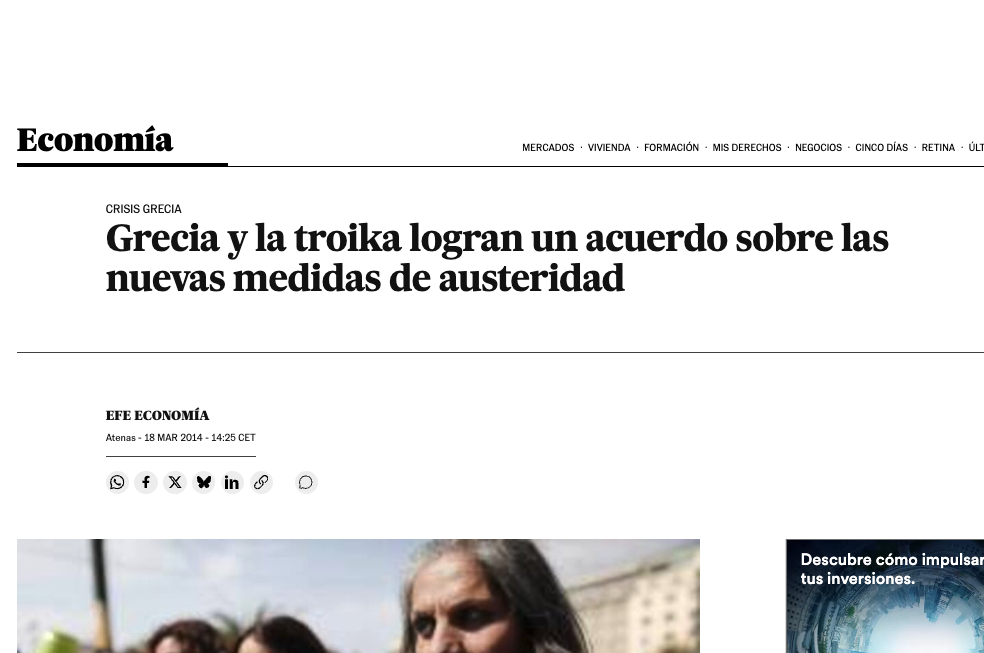
\includegraphics[keepaspectratio, height=\paperheight]{../img/greece_austerity.jpg}};
  \end{tikzpicture}
\end{frame}
% ----------------------------------------------------
% IMAGE NEEDED: greece_austerity.jpg -- fotografía de protestas callejeras en Grecia durante la crisis de deuda (2010-2015), preferiblemente con manifestantes frente al parlamento en la plaza Syntagma de Atenas, o imágenes de colas ante bancos cerrados durante el corralito griego de 2015
\note{Grecia durante la crisis del euro (2010-2015) se convirtió en el símbolo de la austeridad impuesta por la troika (FMI, BCE, Comisión Europea) a cambio de rescates financieros. Las condiciones incluían recortes drásticos en salarios públicos, pensiones, sanidad y educación. El PIB griego cayó un 25\% entre 2008 y 2013, una caída comparable a la Gran Depresión americana. El desempleo llegó al 27\%. Las protestas fueron masivas. La elección de Syriza en 2015 con un mandato anti-austeridad llevó al célebre enfrentamiento entre Varoufakis y el Eurogrupo, y al referéndum del ``No'' de julio de 2015, seguido de la aceptación del tercer rescate. El caso griego ilustra perfectamente la tensión entre la soberanía democrática y las exigencias de los acreedores externos.}

% ----------------------------------------------------
\begin{frame}
\frametitle{El FMI: ¿árbitro o prestamista de último recurso?}
\centering

\begin{itemize}
  \item El \textbf{FMI} (Bretton Woods, 1944): prestamista de último recurso para países en crisis
  \item \textbf{Funciones}:
  \begin{itemize}
    \item Provee información (supervisa datos macroeconómicos) y credibilidad
    \item \textbf{Condicionalidad}: los préstamos exigen ajuste fiscal, reformas, privatizaciones
  \end{itemize}
  \vspace{6pt}
  \item<2-> \textbf{La crítica:} el FMI representa los intereses de los \alert{prestamistas}
  \begin{itemize}
    \item Impone el coste del ajuste sobre los ciudadanos del país deudor
    \item Stiglitz (2002): las recetas del FMI agravan las crisis en lugar de resolverlas
  \end{itemize}
  \vspace{6pt}
  \item<3-> ¿Por qué presta alguien a un soberano que no puede ser embargado?\\
  \small $\rightarrow$ \textbf{Reputación} + el FMI como garante del compromiso
\end{itemize}

\end{frame}
% ----------------------------------------------------
\note{El FMI resuelve dos problemas que hacen difícil el préstamo soberano: (1) Información asimétrica: los prestamistas privados no tienen información fiable sobre las finanzas de los países en desarrollo. El FMI supervisa y certifica esa información, reduciendo el riesgo de que los acreedores presten a gobiernos que están peor de lo que parecen. (2) Compromiso: un gobierno que quiere financiación exterior tiene que comprometerse a políticas responsables. El FMI actúa como garante de ese compromiso: si el gobierno incumple las condiciones, el FMI corta el grifo, lo que señala a los mercados privados que el gobierno no es fiable. La crítica más potente, desarrollada por Stiglitz y otros, es que la condicionalidad del FMI está sesgada hacia los intereses de los acreedores: exige ajuste fiscal (que reduce el consumo) y tipos de interés altos (que atraen capital pero estranGulan la economía), pero no exige a los acreedores que asuman pérdidas. En la crisis asiática de 1997, Stiglitz argumentó que las condiciones del FMI convirtieron una crisis de liquidez en una crisis de solvencia.}

% ----------------------------------------------------
\begin{frame}
\frametitle{Argentina 2001: el mayor impago de la historia}
\centering

\begin{columns}[T]
  \begin{column}{0.52\textwidth}
    \begin{itemize}
      \setlength{\itemsep}{5pt}
      \item Deuda: \textbf{93.000 millones de dólares} (mayor impago soberano de la historia)
      \item Peso anclado al dólar 1:1 desde 1991
      \item Economía no competitiva $\rightarrow$ recesión
      \item Diciembre 2001: \textbf{5 presidentes en 2 semanas}
      \item PIB cayó un \textbf{11\%}; desempleo al \textbf{20\%}
    \end{itemize}
  \end{column}
  \begin{column}{0.44\textwidth}
    \centering
    \vspace{1em}
    {\footnotesize
    \begin{tabular}{lc}
    \textbf{Evento} & \textbf{Año} \\
    \hline
    Convertibilidad 1:1 & 1991 \\
    Crisis brasileña & 1999 \\
    Recesión profunda & 2000--01 \\
    Corralito bancario & Dic.\ 2001 \\
    Impago soberano & Ene.\ 2002 \\
    Devaluación peso & Ene.\ 2002 \\
    Renegociación & 2005--10 \\
    \end{tabular}
    }
  \end{column}
\end{columns}

\end{frame}
% ----------------------------------------------------
\note{La crisis argentina de 2001 es el caso de libro de texto de la interacción entre tipo de cambio fijo, deuda soberana, y colapso político. La convertibilidad (1:1 con el dólar desde 1991) fue inicialmente un éxito: acabó con la hiperinflación de los años 80. Pero ató las manos de la política monetaria y fiscal: cuando el dólar se apreció en los años 90, el peso también se apreció, haciendo las exportaciones argentinas no competitivas. La crisis brasileña de 1999 (devaluación del real) empeoró la situación. Argentina entró en recesión en 1999, el FMI siguió prestando con condiciones de austeridad que agravaron la contracción, y finalmente el sistema colapsó en diciembre de 2001. El corralito (congelación de depósitos bancarios) desencadenó protestas masivas. Argentina tuvo 5 presidentes en dos semanas. El impago de 93.000 millones fue el mayor de la historia hasta entonces. La posterior devaluación del peso (de 1:1 a 3:1 en semanas) destruyó el ahorro de la clase media. La recuperación fue notable (8\% de crecimiento anual 2003-2007), basada en exportaciones agrícolas favorecidas por la devaluación, pero el coste social fue inmenso.}

% ====================================================
\section{Tipos de cambio}
% ====================================================

% ----------------------------------------------------
\begin{transitionframe}
Tipos de cambio y sistemas monetarios
\end{transitionframe}
% ----------------------------------------------------
\note{}

% ----------------------------------------------------
\begin{frame}
\frametitle{¿Qué es el tipo de cambio?}
\centering

\begin{itemize}
  \item El \alert{tipo de cambio} es el precio de una moneda en términos de otra
  \vspace{8pt}
  \item Ejemplos:
  \begin{itemize}
    \item 1 euro = 1,10 dólares
    \item Si el euro \textbf{se aprecia}: 1 euro = 1,20 dólares (más dólares por euro)
    \item Si el euro \textbf{se deprecia}: 1 euro = 0,95 dólares (menos dólares por euro)
  \end{itemize}
  \vspace{8pt}
  \item<2-> ¿Por qué importa? --- Ejemplo concreto:
  \begin{itemize}
    \item Con un euro fuerte, el hotel en Roma te \textbf{sale más barato} si eres americano
    \item Los coches alemanes se vuelven \textbf{más caros} para los americanos
    \item Las exportaciones españolas se hacen \textbf{menos competitivas}
  \end{itemize}
\end{itemize}

\end{frame}
% ----------------------------------------------------
\note{El tipo de cambio es quizás la variable económica que más afecta a la vida cotidiana de las personas sin que sean conscientes de ello. Afecta al precio de las importaciones (y por tanto a la inflación), a la competitividad de las exportaciones, al valor real de la deuda externa (si un país tiene deuda en dólares y su moneda se deprecia, la deuda se vuelve más pesada en términos reales), y al flujo de turistas. Para entender la política de los tipos de cambio es útil el ejemplo del turista: si el euro se aprecia frente al dólar, los europeos que van a EE.UU. se encuentran con que todo es más barato (sus euros compran más dólares), pero los americanos que vienen a Europa encuentran todo más caro. Esto beneficia a las empresas turísticas americanas y perjudica a las europeas.}

% ----------------------------------------------------
\begin{frame}
\frametitle{¿Quién gana y quién pierde?}
\centering
\vspace{0.5em}

{\footnotesize
\begin{adjustbox}{width=\textwidth}
\begin{tabular}{>{\bfseries}p{3cm} p{2.8cm} p{2.8cm}}
 & \textbf{\textcolor{accent}{Moneda fuerte (apreciación)}} & \textbf{\textcolor{accent2}{Moneda débil (depreciación)}} \\[6pt]
\hline
Consumidores & Importaciones baratas & Importaciones caras, inflación \\[5pt]
Exportadores & Pierden competitividad & Ganan competitividad \\[5pt]
Turismo receptor & Menos turistas & Más turistas \\[5pt]
Deuda en \$\,/\,\texteuro{} & Más fácil de pagar & Más pesada \\[5pt]
Sector financiero & Prefiere estabilidad & Volatilidad, riesgo \\[5pt]
\end{tabular}
\end{adjustbox}
}

\vspace{8pt}
\onslide<2->{\small El tipo de cambio es \textbf{distributivamente conflictivo}: crea ganadores y perdedores dentro de cada país}

\end{frame}
% ----------------------------------------------------
\note{La tabla resume los efectos distributivos del tipo de cambio. El punto central: no existe un tipo de cambio ``bueno'' en abstracto, porque siempre hay ganadores y perdedores. Una moneda fuerte beneficia a los consumidores (importaciones baratas, viajes al exterior asequibles) y al sector financiero (estabilidad), pero perjudica a los exportadores. Una moneda débil beneficia a los exportadores y atrae turismo, pero genera inflación que golpea sobre todo a los más pobres. Esto explica por qué la política cambiaria es siempre políticamente conflictiva. En Alemania, el Bundesbank tenía una obsesión con la estabilidad del marco y el control de la inflación (herencia de la hiperinflación de los años 20). En países exportadores como Japón o China, los gobiernos han preferido mantener su moneda relativamente depreciada para favorecer las exportaciones. EE.UU. ha acusado repetidamente a China de manipular su moneda para obtener ventaja competitiva desleal.}

% ----------------------------------------------------
\begin{frame}
\frametitle{El trilema de la política monetaria}
\centering
\vspace{0.2em}

\begin{tikzpicture}[>=stealth, scale=0.9]
  % Triangle vertices
  \coordinate (A) at (0, 3.5);   % top: tipo fijo
  \coordinate (B) at (-3.5, 0);  % bottom-left: libre capital
  \coordinate (C) at (3.5, 0);   % bottom-right: pol. monetaria

  % Triangle sides
  \draw[thick] (A) -- (B) -- (C) -- cycle;

  % Vertex labels
  \node[above, font=\small\bfseries] at (A) {Tipo de cambio fijo};
  \node[left, font=\small\bfseries, align=right] at (B) {Libre movimiento\\de capitales};
  \node[right, font=\small\bfseries, align=left] at (C) {Política monetaria\\autónoma};

  % Country examples on each side (which two you pick)
  \node[left, font=\scriptsize, text=accent, align=center] at (-1.75, 1.75)
    {Eurozona\\(fijo + libre capital)};
  \node[below, font=\scriptsize, text=asher, align=center] at (0, -0.15)
    {EE.UU. / UK (libre capital + pol. monetaria)};
  \node[right, font=\scriptsize, text=accent2, align=center] at (1.75, 1.75)
    {China 2000s\\(fijo + pol. monetaria)};
\end{tikzpicture}

\vspace{4pt}
{\small \alert{Solo puedes elegir dos de los tres:} cada par excluye el tercero}

\end{frame}
% ----------------------------------------------------
\note{El trilema (o trinidad imposible) de la política monetaria es uno de los conceptos más importantes de la economía internacional. Dice que un país solo puede tener dos de las tres siguientes cosas al mismo tiempo: (1) tipo de cambio fijo, (2) libre movimiento de capitales, y (3) política monetaria autónoma. Si tienes tipo fijo y libre movimiento de capitales, tu política monetaria debe estar supeditada a mantener la paridad (como pasó en Argentina). Si tienes libre movimiento de capitales y política monetaria autónoma, el tipo de cambio debe flotar. Si quieres tipo fijo y política monetaria autónoma, tienes que controlar los capitales (como hacía China hasta los años 2000). Esta restricción explica muchas de las tensiones de la política económica internacional. Los países de la eurozona han elegido tipo fijo (moneda única) y libre movimiento de capitales, renunciando a la política monetaria nacional.}

% ----------------------------------------------------
\begin{frame}
\frametitle{Evolución del sistema monetario internacional}
\centering
\vspace{0.5em}

\begin{tikzpicture}[>=stealth, thick]
  % Timeline base
  \draw[thick] (0,0) -- (10,0);

  % Period bands below
  \fill[accent!25] (0,-0.8) rectangle (3,-0.3);
  \fill[accent2!20] (3,-0.8) rectangle (4.5,-0.3);
  \fill[accent!15] (4.5,-0.8) rectangle (7,-0.3);
  \fill[asher!20] (7,-0.8) rectangle (10,-0.3);

  % Period labels
  \node[font=\scriptsize, align=center] at (1.5,-0.55) {Patrón oro};
  \node[font=\scriptsize, align=center] at (3.75,-0.55) {Entreguerras};
  \node[font=\scriptsize, align=center] at (5.75,-0.55) {Bretton Woods};
  \node[font=\scriptsize, align=center] at (8.5,-0.55) {Flotación / Euro};

  % Ticks above
  \foreach \x/\lab in {0/1870, 3/1914, 4.5/1944, 7/1973, 8.5/1999} {
    \draw (\x, -0.1) -- (\x, 0.25);
    \node[above, font=\scriptsize] at (\x, 0.2) {\lab};
  }

  % Event labels above
  \node[above, font=\scriptsize, align=center, text=accent] at (1.5, 0.5) {Estabilidad\\y deflación};
  \node[above, font=\scriptsize, align=center, text=accent2] at (3.75, 0.5) {Caos y\\guerras};
  \node[above, font=\scriptsize, align=center, text=accent] at (5.75, 0.5) {\$=oro\\35\$/oz};
  \node[above, font=\scriptsize, align=center, text=asher] at (8.5, 0.5) {Nixon shock\\$\rightarrow$ euro};
\end{tikzpicture}

\end{frame}
% ----------------------------------------------------
\note{La historia del sistema monetario internacional es una historia de intentos de resolver el trilema de forma diferente. El patrón oro (1870-1914): todas las monedas están fijas al oro, lo que garantiza estabilidad cambiaria. El problema: la oferta monetaria depende de las reservas de oro, lo que es deflacionario en períodos de crecimiento. El período de entreguerras: el abandono del patrón oro durante la Primera Guerra Mundial, el retorno parcial en los años 20, y el colapso final en la Gran Depresión. Los países comenzaron a depreciar sus monedas competitivamente (``beggar thy neighbor''), lo que agravó la crisis global. Bretton Woods (1945-73): el dólar como ancla (convertible en oro a 35 dólares por onza), otras monedas fijas al dólar pero ajustables. Funcionó bien durante los ``Treinta Gloriosos'', pero la inflación americana de los años 60 (provocada por el gasto en Vietnam y los programas sociales de Johnson) hizo insostenible la paridad. Nixon cerró la ventanilla del oro en 1971 (el ``Nixon shock''), y en 1973 las principales monedas comenzaron a flotar. Desde entonces el sistema es de flotación administrada para las grandes divisas, con muchos países más pequeños que fijan su moneda al dólar o al euro.}

% ----------------------------------------------------
\begin{frame}
\frametitle{El euro: integración sin soberanía monetaria}
\centering

\begin{itemize}
  \item 20 países de la UE comparten el euro desde 1999--2002
  \vspace{8pt}
  \item \textbf{Ventajas:}
  \begin{itemize}
    \item Elimina el riesgo cambiario dentro de la eurozona
    \item Reduce costes de transacción (un solo mercado)
    \item Credibilidad antiinflacionaria (BCE independiente)
  \end{itemize}
  \vspace{8pt}
  \item<2-> \textbf{El coste:} pérdida de \alert{soberanía monetaria}
  \begin{itemize}
    \item No puedes devaluar para recuperar competitividad
    \item No puedes fijar tipos de interés según tu ciclo económico
    \item Una sola política monetaria para economías muy diferentes
  \end{itemize}
  \item<3-> \textbf{El problema:} Alemania y Grecia no son la misma economía
\end{itemize}

\end{frame}
% ----------------------------------------------------
\note{La creación del euro fue la apuesta política más ambiciosa de la integración europea. La teoría del Área Monetaria Óptima (Mundell, 1961) establece las condiciones bajo las que tiene sentido compartir moneda: movilidad laboral, flexibilidad salarial, transferencias fiscales entre regiones. La eurozona cumple algunas de estas condiciones, pero no todas. La movilidad laboral en Europa es baja comparada con EE.UU. No hay transferencias fiscales significativas (no hay presupuesto europeo digno de ese nombre). Y las economías son muy heterogéneas: Alemania tiene superávit por cuenta corriente crónico, mientras que países del sur tenían déficits crónicos antes de la crisis. Cuando llegó el shock de 2008, países como España o Grecia no podían depreciar su moneda para recuperar competitividad (eso se hace automáticamente con moneda propia), y solo podían ajustar a través de la ``devaluación interna'': bajar salarios y precios, lo que es enormemente doloroso socialmente. El euro sobrevivió, pero a un coste político muy alto.}

% ====================================================
\section{Crisis monetarias}
% ====================================================

% ----------------------------------------------------
\begin{transitionframe}
Crisis monetarias y contagio
\end{transitionframe}
% ----------------------------------------------------
\note{}

% ----------------------------------------------------
\begin{frame}
\frametitle{¿Cómo ocurre una crisis monetaria?}
\centering
\vspace{0.3em}

\begin{tikzpicture}[>=stealth, thick, node distance=1.6cm]
  \node[draw, fill=accent!15, rounded corners, minimum width=3.5cm, minimum height=0.8cm, align=center, font=\small] (start) at (5, 4.5)
    {Tipo de cambio fijo};
  \node[draw, fill=accent2!10, rounded corners, minimum width=3.5cm, minimum height=0.8cm, align=center, font=\small] (doubt) at (5, 3.1)
    {Inversores dudan de la paridad};
  \node[draw, fill=accent2!20, rounded corners, minimum width=3.5cm, minimum height=0.8cm, align=center, font=\small] (attack) at (5, 1.7)
    {Ataque especulativo: venden moneda};
  \node[draw, fill=accent2!30, rounded corners, minimum width=3.5cm, minimum height=0.8cm, align=center, font=\small] (reserves) at (5, 0.3)
    {Se agotan las reservas del banco central};
  \node[draw, fill=accent2!50, rounded corners, minimum width=3.5cm, minimum height=0.8cm, align=center, font=\small] (collapse) at (5, -1.1)
    {\textbf{Colapso: devaluación o flotación}};

  \draw[->] (start) -- (doubt);
  \draw[->] (doubt) -- (attack);
  \draw[->] (attack) -- (reserves);
  \draw[->] (reserves) -- (collapse);

  \node[font=\scriptsize, text=accent2, align=center] at (8.2, 1.7) {\textit{Profecía}\\\textit{autocumplida}};
  \draw[->, dashed, accent2] (7.9, 2.1) -- (6.8, 2.4);
\end{tikzpicture}

\end{frame}
% ----------------------------------------------------
\note{Las crisis monetarias tienen una lógica de profecía autocumplida. Un gobierno puede mantener un tipo de cambio fijo mientras los mercados crean que puede y quiere hacerlo. Pero si los inversores comienzan a dudar de la paridad, atacan: venden masivamente la moneda local y compran divisas extranjeras. El banco central tiene que usar sus reservas de divisas para comprar su propia moneda y defender la paridad. Cuando las reservas se agotan, el gobierno no puede sostener el tipo de cambio y se produce la devaluación. El punto crucial: la crisis puede ocurrir aunque las ``fundamentales'' de la economía sean razonables, porque si suficientes inversores creen que la moneda caerá, su comportamiento colectivo causa exactamente esa caída. George Soros es el ejemplo más famoso: en 1992 apostó 10.000 millones de dólares contra la libra esterlina dentro del Sistema Monetario Europeo (el mecanismo que precedió al euro). La libra cayó, Soros ganó 1.000 millones en un día, y el Reino Unido tuvo que salir del SME.}

% ----------------------------------------------------
\begin{frame}
\frametitle{La crisis del euro: deuda soberana y contagio}
\centering

\begin{itemize}
  \item \textbf{2008-2015:} crisis de deuda soberana en la eurozona
  \vspace{6pt}
  \item Países afectados: \textbf{Grecia, Irlanda, Portugal, España, Chipre}
  \vspace{6pt}
  \item Mecanismo:
  \begin{itemize}
    \item Crisis financiera global 2008 $\rightarrow$ recesión $\rightarrow$ déficits públicos
    \item Mercados dudan de la solvencia $\rightarrow$ \textbf{prima de riesgo} (sobrecoste de financiación) sube
    \item Rescates: troika (FMI + BCE + Comisión) impone condiciones
  \end{itemize}
  \vspace{6pt}
  \item<2-> \textbf{El problema del euro:} no puede haber crisis de tipo de cambio, pero sí crisis de deuda soberana
  \begin{itemize}
    \item Sin devaluación posible: solo queda la ``devaluación interna''
    \item Consecuencia: austeridad profunda y recesión prolongada
  \end{itemize}
  \item<3-> \alert{Mario Draghi (2012):} ``Whatever it takes'' --- el BCE compra deuda
\end{itemize}

\end{frame}
% ----------------------------------------------------
\note{La crisis del euro de 2010-2015 es una de las grandes pruebas de la integración europea. Comenzó con la revelación de que Grecia había falsificado sus estadísticas fiscales (el déficit real era mucho mayor de lo declarado). Los mercados comenzaron a cobrar primas de riesgo crecientes a Grecia, y el contagio se extendió a Irlanda (que había rescatado sus bancos con dinero público), Portugal, España y Chipre. Los tres rescates griegos (2010, 2012, 2015) totalizaron más de 300.000 millones de euros, con condiciones de austeridad draconiana. El momento crítico fue julio de 2012, cuando Draghi anunció que el BCE haría ``todo lo que sea necesario'' para preservar el euro. Esto calmó los mercados sin que el BCE tuviera que comprar un solo bono en ese momento: la sola promesa fue suficiente. La lección: la credibilidad es la herramienta más potente de la política monetaria. El Brexit en 2016 fue parcialmente una reacción política al malestar con la austeridad y la percepción de que la UE prioriza los intereses financieros sobre los ciudadanos.}

% ----------------------------------------------------
\begin{frame}
\frametitle{Contagio: cómo se propagan las crisis}
\centering
\vspace{0.5em}

\begin{columns}[T]
  \begin{column}{0.5\textwidth}
    \textbf{Crisis asiática (1997)}
    \begin{itemize}
      \item Julio: colapso del baht tailandés
      \item Agosto: ringgit malayo
      \item Octubre: won coreano
      \item Noviembre: rupia indonesia
      \item FMI rescata con condiciones duras
    \end{itemize}
  \end{column}
  \begin{column}{0.46\textwidth}
    \textbf{Mecanismos de contagio}
    \begin{itemize}
      \item Vínculos comerciales: si el vecino colapsa, tus exportaciones caen
      \item Vínculos financieros: bancos expuestos a varios países
      \item Pánico de inversores: ``si Tailandia cayó, Corea puede caer''
      \item Profecía autocumplida regional
    \end{itemize}
  \end{column}
\end{columns}

\vspace{10pt}
\onslide<2->{\small Las finanzas globales \textbf{amplifican} los shocks: lo que empieza en Bangkok llega a Seúl en semanas}

\end{frame}
% ----------------------------------------------------
\note{El contagio financiero es uno de los fenómenos más perturbadores de la globalización financiera. En 1997, la crisis comenzó con la devaluación del baht tailandés en julio. En semanas, los inversores comenzaron a retirar capital de otros países de la región (Malasia, Indonesia, Corea del Sur, Filipinas), anticipando que sufrirían los mismos problemas. Fue en parte una profecía autocumplida: la retirada de capitales provocó exactamente la crisis que los inversores temían. En Indonesia, la crisis fue especialmente devastadora: el PIB cayó un 13\%, el desempleo masivo, y el malestar político llevó a la caída de Suharto tras 32 años en el poder. Las condiciones del FMI en Asia en 1997 son el caso de estudio más debatido sobre la condicionalidad. El FMI exigió austeridad fiscal y tipos de interés altos en países que ya estaban en crisis de confianza, lo que muchos economistas creen que agravó el contagio. Stiglitz, entonces economista jefe del Banco Mundial, publicó una crítica devastadora que le costó el puesto pero que la comunidad académica en gran parte validó.}

% ----------------------------------------------------
\begin{frame}[plain]
  \begin{tikzpicture}[remember picture, overlay]
    \node[at = (current page.center), yshift = 0cm] (cover) {%
      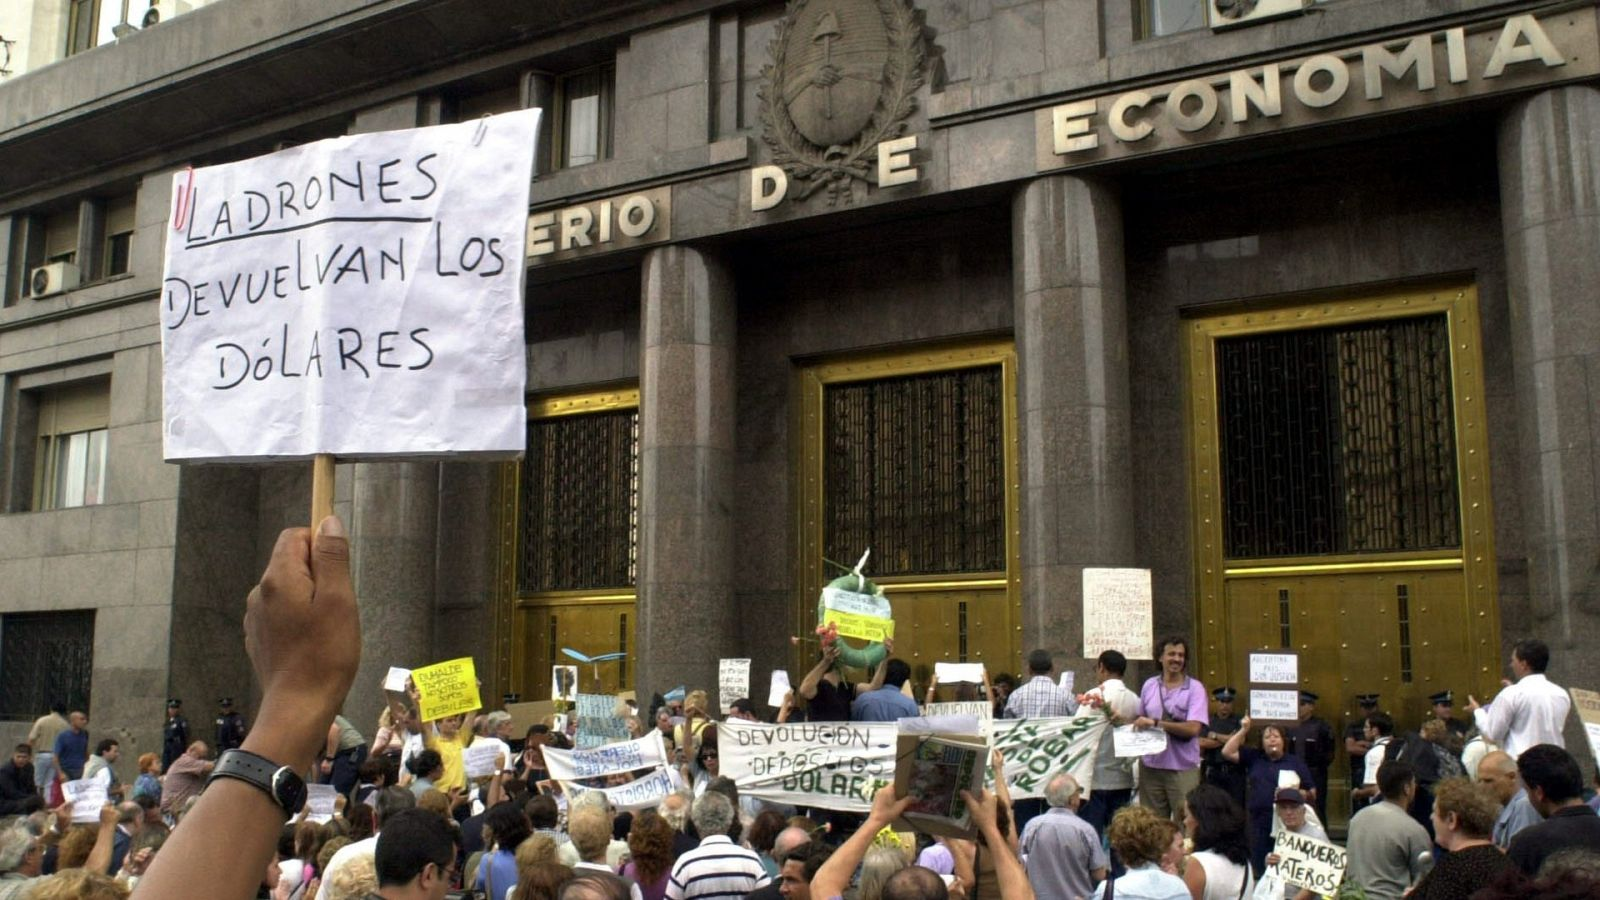
\includegraphics[keepaspectratio, height=\paperheight]{../img/argentina_2001.jpg}};
  \end{tikzpicture}
\end{frame}
% ----------------------------------------------------
% IMAGE NEEDED: argentina_2001.jpg -- fotografía de las protestas y disturbios en Buenos Aires en diciembre de 2001, preferiblemente con imágenes de ciudadanos golpeando cacerolas (cacerolazos), o de las largas colas ante los bancos cerrados por el corralito, o de la renuncia del presidente De la Rúa
\note{Las imágenes de Argentina en diciembre de 2001 son icónicas de lo que una crisis de deuda y monetaria puede hacer a una sociedad. El corralito (congelación de los depósitos bancarios) impidió a los ciudadanos acceder a sus propios ahorros. Los cacerolazos -- ciudadanos de clase media golpeando cacerolas en las calles -- se convirtieron en el símbolo de la protesta. El presidente Fernando de la Rúa tuvo que abandonar el palacio presidencial en helicóptero. La cadena de presidentes interinos fue de una velocidad vertiginosa: cinco en dos semanas. El default se declaró en enero de 2002. La recuperación posterior fue notable, pero el trauma social y político duró décadas. Argentina es todavía hoy el país que más veces ha entrado en default soberano en la historia moderna.}

% ----------------------------------------------------
\begin{frame}
\frametitle{Resumen}
\centering
\vspace{1em}

\begin{itemize}
  \setlength{\itemsep}{8pt}
  \item La inversión internacional fluye donde rinde más, pero el \textbf{riesgo político} distorsiona ese flujo
  \item La IED la realizan \textbf{multinacionales}; la reshoring y friendshoring reflejan tensiones geopolíticas
  \item La \textbf{deuda soberana} genera conflictos distributivos: ¿quién paga el ajuste?
  \item El \textbf{FMI} resuelve problemas de información y compromiso, pero impone condicionalidad
  \item Los tipos de cambio crean \textbf{ganadores y perdedores} dentro de cada país
  \item El \textbf{trilema monetario}: no puedes tener tipo fijo, libre capital y política monetaria propia
  \item Las crisis \textbf{se contagian}: la globalización financiera amplifica los shocks
\end{itemize}

\end{frame}
% ----------------------------------------------------
\note{Resumen integrador de los conceptos de la sesión. El hilo conductor es que cada dimensión de las finanzas internacionales --- inversión, deuda, tipos de cambio, crisis --- tiene una estructura distributiva: hay ganadores y perdedores, y la política determina quién carga con los costes. La inversión favorece a los países con bajo riesgo político. La deuda soberana enfrenta a prestamistas con deudores y ciudadanos. Los tipos de cambio dividen a exportadores de consumidores. Las crisis financieras se contagian y a menudo el coste lo pagan los más vulnerables. El FMI es una institución que intenta gestionar estas tensiones, pero que refleja la correlación de fuerzas entre acreedores y deudores en el sistema internacional. Argentina y Grecia son los dos casos de referencia para ilustrar cómo estos mecanismos funcionan en la práctica.}

% ----------------------------------------------------
\begin{frame}
\centering
\vspace{2em}
{\large ¿Es posible tener integración financiera global\\[10pt]
sin un prestamista de último recurso global\\[6pt]
que responda ante los ciudadanos?}
\end{frame}
% ----------------------------------------------------
\note{Pregunta de cierre para debate. El FMI es el prestamista de último recurso de facto del sistema internacional, pero no responde democráticamente ante los ciudadanos de los países que rescata. Sus cuotas de voto están dominadas por los países ricos (EE.UU. tiene poder de veto). La propuesta de un prestamista de último recurso global genuinamente representativo existe en la teoría, pero no en la práctica. Alternativas: la posibilidad de que el BCE actuara como prestamista de último recurso para la eurozona (lo que Draghi hizo en 2012 con el ``whatever it takes''). La pregunta conecta con el debate más amplio sobre la gobernanza global: ¿puede existir una economía global sin instituciones globales con legitimidad democrática? ¿O estamos condenados al dilema entre integración económica y soberanía democrática?}
